\subsection{Package sequenziatore::server::model}
\begin{figure}[H] \centering 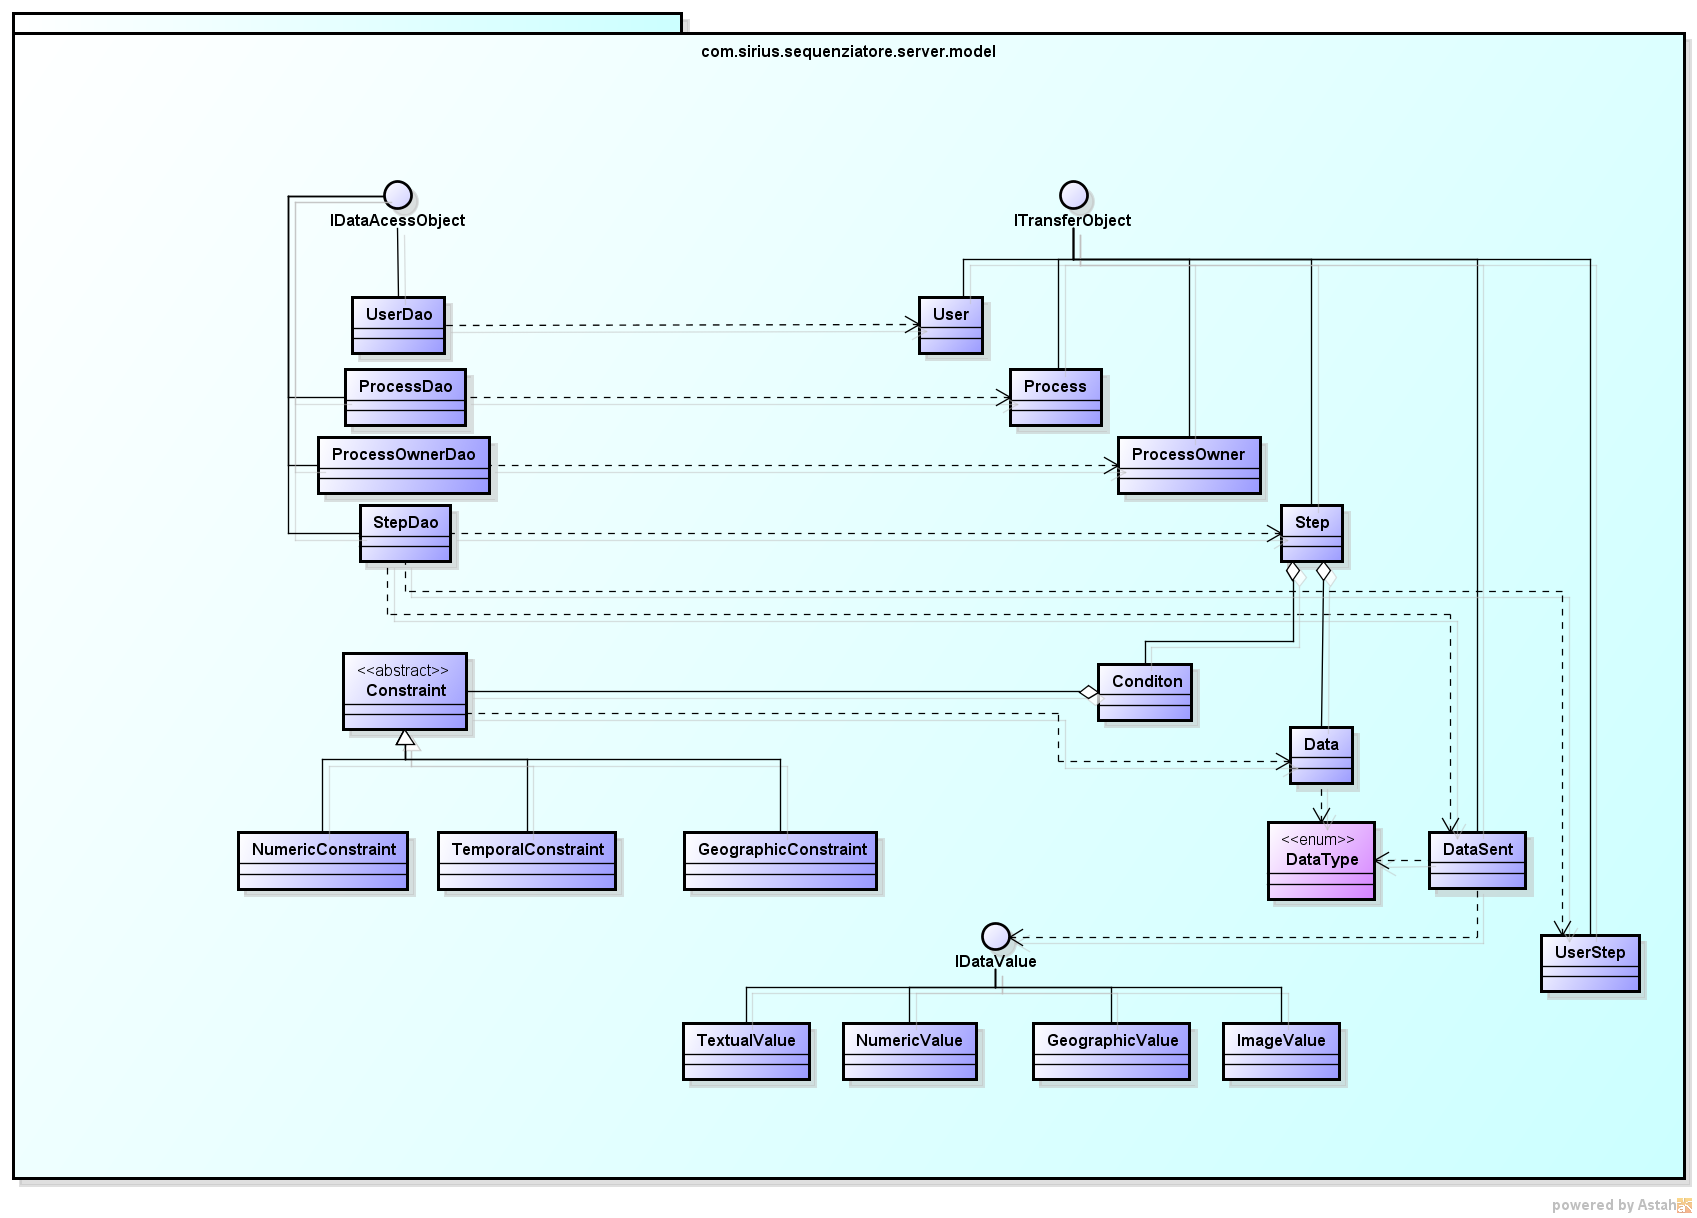
\includegraphics[width=%
\textwidth]
{./pack/ClassiServerSoloModel.png} \caption{Diagramma model server}
\end{figure}
\paragraph{DaoFacade}
	\begin{itemize}
		\item \textbf{Nome:} \texttt{DaoFacade};
		\item \textbf{Tipo:} abstract;
		\item \textbf{Package:} sequenziatore::server::model
		\item \textbf{Descrizione:} Classe astratta che decide a che pacchetto assegnare la richiesta di esecuzione \textit{query};
		\item \textbf{Relazione con altre componenti:} la classe invoca i metodi delle seguenti classi:
		\begin{itemize}
			\item sequenziatore::server::model::daoprocessowner::ObjectTransfer tramite l' interfaccia sequenziatore::server::model::daoprocessowner::IObjectTransfer
			\item sequenziatore::server::model::daoprocessowner::DataAccessObject tramite l' interfaccia sequenziatore::server::model::daoprocessowner::IDataAccessObject
			\item sequenziatore::server::model::daostep::ObjectTransfer tramite l' interfaccia sequenziatore::server::model::daostep::IObjectTransfer
			\item sequenziatore::server::model::daostep::DataAccessObject tramite l' interfaccia sequenziatore::server::model::daostep::IDataAccessObject
			\item sequenziatore::server::model::daouser::ObjectTransfer tramite l' interfaccia sequenziatore::server::model::daouser::IObjectTransfer
			\item sequenziatore::server::model::daouser::DataAccessObject tramite l' interfaccia sequenziatore::server::model::daouser::IDataAccessObject
			\item sequenziatore::server::model::daoprocess::ObjectTransfer tramite l' interfaccia sequenziatore::server::model::daoprocess::IObjectTransfer
			\item sequenziatore::server::model::daoprocess::DataAccessObject tramite l' interfaccia sequenziatore::server::model::daoprocess::IDataAccessObject
		\end{itemize}
	\end{itemize}
\subsubsection{Package sequenziatore::server::model::daouser}
\paragraph{IDataAccessObject}
	\begin{itemize}
		\item \textbf{Nome:} \texttt{IDataAccessObject};
		\item \textbf{Package:} sequenziatore::server::model::daouser
		\item \textbf{Descrizione:} Interfaccia con il compito di interagire con il database.
	\end{itemize}
%------------------------------------------------------------------------------%
\paragraph{DataAccessObject}
	\begin{itemize}
		\item \textbf{Nome:} \texttt{DataAccessObject};
		\item \textbf{Package:} sequenziatore::server::model::daouser
		\item \textbf{Descrizione:} classe che si occupa di effettuare le richieste al database, acquisendo i dati richiesti o inserendone di nuovi.
		\item \textbf{Relazione con altre componenti:} la classe implementa l' interfaccia sequenziatore::server::model::daouser::IDataAccessObject ed invoca metodi delle classi:
		\begin{itemize}
			\item sequenziatore::server::model::daouser::ObjectTransfer tramite l' interfaccia sequenziatore::server::model::daouser::IObjectTransfer
		\end{itemize}
	\end{itemize}
	%------------------------------------------------------------------------------%
\paragraph{IObjectTransfer}
	\begin{itemize}
		\item \textbf{Nome:} \texttt{IObjectTransfer};
		\item \textbf{Package:} sequenziatore::server::model::daouser
		\item \textbf{Descrizione:} Interfaccia che permette lo scambio di dati tra model e presenter.
	\end{itemize}
	%------------------------------------------------------------------------------%
\paragraph{ObjectTransfer}
	\begin{itemize}
		\item \textbf{Nome:} \texttt{ObjectTransfer};
		\item \textbf{Package:} sequenziatore::server::model::daouser
		\item \textbf{Descrizione:} Classe che permette lo scambio di dati tra la classe DataAccessObject e il presenter.
		\item \textbf{Relazione con altre componenti:} la classe implementa l'interfaccia sequenziatore::server::model::daouser::IObjectTransfer.
	\end{itemize}
%000000000000000000000000000000000000000000000000000000000000000000000000000000000000%
\subsubsection{Package sequenziatore::server::model::daoprocessowner}
\paragraph{IDataAccessObject}
	\begin{itemize}
		\item \textbf{Nome:} \texttt{IDataAccessObject};
		\item \textbf{Package:} sequenziatore::server::model::daoprocessowner
		\item \textbf{Descrizione:} Interfaccia con il compito di interagire con il database.
	\end{itemize}
	%------------------------------------------------------------------------------%
\paragraph{DataAccessObject}
\begin{itemize}
		\item \textbf{Nome:} \texttt{DataAccessObject};
		\item \textbf{Package:} sequenziatore::server::model::daoprocessowner
		\item \textbf{Descrizione:} classe che si occupa di effettuare le richieste al database, acquisendo i dati richiesti o inserendone di nuovi.
		\item \textbf{Relazione con altre componenti:} la classe implementa l' interfaccia sequenziatore::server::model::daoprocessowner::IDataAccessObject ed invoca metodi delle classi:
		\begin{itemize}
			\item sequenziatore::server::model::daoprocessowner::ObjectTransfer tramite l' interfaccia sequenziatore::server::model::daoprocessowner::IObjectTransfer
		\end{itemize}
\end{itemize}
	%------------------------------------------------------------------------------%
\paragraph{IObjectTransfer}
	\begin{itemize}
		\item \textbf{Nome:} \texttt{IObjectTransfer};
		\item \textbf{Package:} sequenziatore::server::model::daoprocessowner
		\item \textbf{Descrizione:} Interfaccia che permette lo scambio di dati tra model e presenter.
	\end{itemize}
	%------------------------------------------------------------------------------%
\paragraph{ObjectTransfer}
	\begin{itemize}
		\item \textbf{Nome:} \texttt{ObjectTransfer};
		\item \textbf{Package:} sequenziatore::server::model::daoprocessowner
		\item \textbf{Descrizione:} Classe che permette lo scambio di dati tra la classe DataAccessObject e il presenter.
		\item \textbf{Relazione con altre componenti:} la classe implementa l'interfaccia sequenziatore::server::model::daoprocessowner::IObjectTransfer.
	\end{itemize}
%000000000000000000000000000000000000000000000000000000000000000000000000000000000000%
\subsubsection{Package sequenziatore::server::model::daoprocess}
\paragraph{IDataAccessObject}
	\begin{itemize}
		\item \textbf{Nome:} \texttt{IDataAccessObject};
		\item \textbf{Package:}sequenziatore::server::model::daoprocess
		\item \textbf{Descrizione:} Interfaccia con il compito di interagire con il database.
	\end{itemize}
	%------------------------------------------------------------------------------%
\paragraph{DataAccessObject}
	\begin{itemize}
		\item \textbf{Nome:} \texttt{DataAccessObject};
		\item \textbf{Package:} sequenziatore::server::model::daoprocess
		\item \textbf{Descrizione:} classe che si occupa di effettuare le richieste al database, acquisendo i dati richiesti o inserendone di nuovi.
		\item \textbf{Relazione con altre componenti:} la classe implementa l' interfaccia sequenziatore::server::model::daoprocess::IDataAccessObject ed invoca metodi delle classi:
		\begin{itemize}
			\item sequenziatore::server::model::daoprocess::ObjectTransfer tramite l' interfaccia sequenziatore::server::model::daoprocess::IObjectTransfer
	\end{itemize}
\end{itemize}
	%------------------------------------------------------------------------------%
\paragraph{IObjectTransfer}
	\begin{itemize}
		\item \textbf{Nome:} \texttt{IObjectTransfer};
		\item \textbf{Package:} sequenziatore::server::model::daoprocess
		\item \textbf{Descrizione:} Interfaccia che permette lo scambio di dati tra model e presenter.
	\end{itemize}
	%------------------------------------------------------------------------------%
\paragraph{ObjectTransfer}
	\begin{itemize}
		\item \textbf{Nome:} \texttt{ObjectTransfer};
		\item \textbf{Package:} sequenziatore::server::model::daoprocess
		\item \textbf{Descrizione:} Classe che permette lo scambio di dati tra la classe DataAccessObject e il presenter.
		\item \textbf{Relazione con altre componenti:} la classe implementa l'interfaccia sequenziatore::server::model::daoprocess::IObjectTransfer.
	\end{itemize}
%000000000000000000000000000000000000000000000000000000000000000000000000000000000000%
\subsubsection{Package sequenziatore::server::model::daostep}
\paragraph{IDataAccessObject}
	\begin{itemize}
		\item \textbf{Nome:} \texttt{IDataAccessObject};
		\item \textbf{Package:} sequenziatore::server::model::daostep
		\item \textbf{Descrizione:} Interfaccia con il compito di interagire con il database.
	\end{itemize}
	%------------------------------------------------------------------------------%
\paragraph{DataAccessObject}
	\begin{itemize}
		\item \textbf{Nome:} \texttt{DataAccessObject};
		\item \textbf{Package:} sequenziatore::server::model::daostep
		\item \textbf{Descrizione:} classe che si occupa di effettuare le richieste al database, acquisendo i dati richiesti o inserendone di nuovi.
		\item \textbf{Relazione con altre componenti:} la classe implementa l' interfaccia sequenziatore::server::model::daostep::IDataAccessObject ed invoca metodi delle classi:
		\begin{itemize}
			\item sequenziatore::server::model::daostep::ObjectTransfer tramite l' interfaccia sequenziatore::server::model::daostep::IObjectTransfer
	\end{itemize}
	\end{itemize}
	%------------------------------------------------------------------------------%
\paragraph{IObjectTransfer}
	\begin{itemize}
		\item \textbf{Nome:} \texttt{IObjectTransfer};
		\item \textbf{Package:} sequenziatore::server::model::daostep
		\item \textbf{Descrizione:} Interfaccia che permette lo scambio di dati tra model e presenter.
	\end{itemize}
	%------------------------------------------------------------------------------%
\paragraph{ObjectTransfer}
	\begin{itemize}
		\item \textbf{Nome:} \texttt{ObjectTransfer};
		\item \textbf{Package:} sequenziatore::server::model::daostep
		\item \textbf{Descrizione:} Classe che permette lo scambio di dati tra la classe DataAccessObject e il presenter.
		\item \textbf{Relazione con altre componenti:} la classe implementa l'interfaccia sequenziatore::server::model::daostep::IObjectTransfer.
	\end{itemize}